%!TEX root = ../main.tex

\graphicspath{{./figures/chapter5/}}

\chapter{Localizing mRNAs}
\label{ch:chapter5}

\minitoc
\newpage

\begin{center}
	\textit{(To be completed)}
\end{center}

\section{General pattern recognition}
\label{sec:general_pattern_recognition}

\begin{center}
	\textit{(To be completed)}
\end{center}

\subsection{Introduction}
\label{subsec:introduction_general_pattern}

\subsection{Materials and methods}
\label{subsec:materials_general_pattern}

\subsubsection{Experimental data}

\begin{figure}[h]
    \centering
    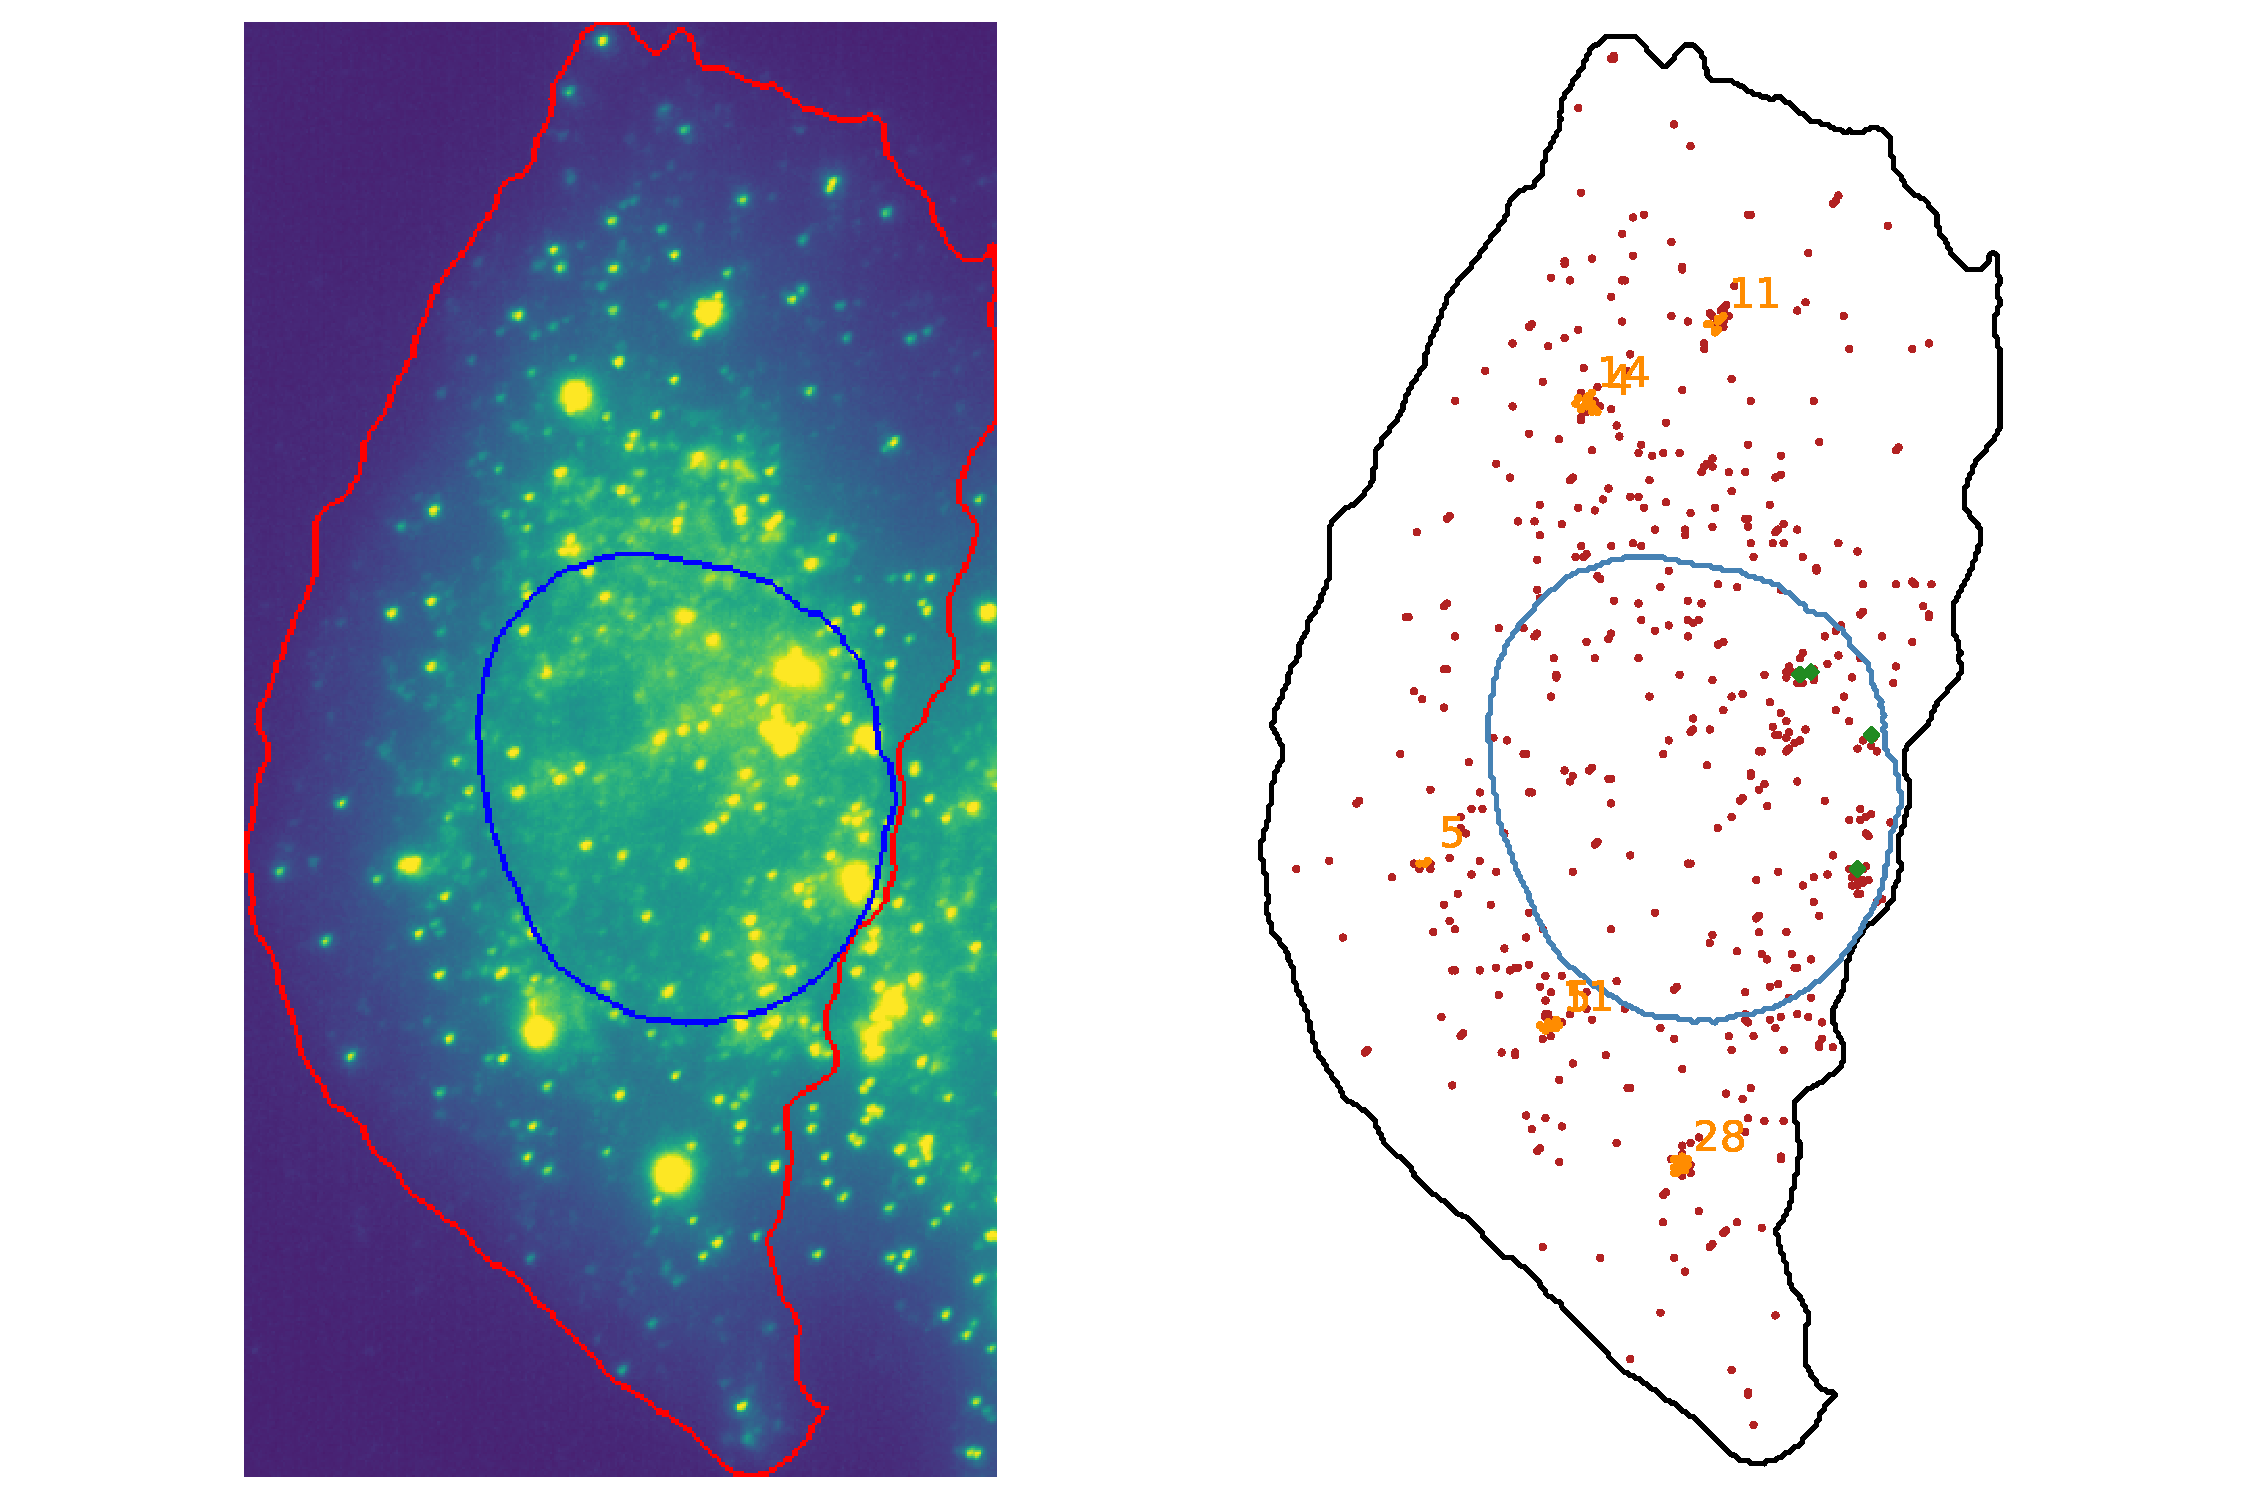
\includegraphics[width=\textwidth]{figures/chapter4/cell_extracted_0}
    \caption{Contrasted original image with segmented boundaries (\textit{left}) and coordinate representation (\textit{right}).
	Plot build with \emph{bigfish}}
    \label{fig:cell_extracted_0}
\end{figure}

\subsubsection{Semi-automated RNA detection}

Image Analysis and Quantifications
Nuclear segmentation was performed from the DAPI channel, cell segmentation from the autofluorescence of the actual smFISH im- age. Prior to segmentation, 3D images were projected to 2D images using maximal local focus values (Tsanov et al., 2016). Nuclei were segmented with a Deep Neural Network (Matterport implementation of the Mask R-CNN, He et al., 2017), trained on the Data Science Bowl 2018. Cells were segmented with a custom algorithm, based on prefiltering the 2D projected smiFISH image, followed by a watershed based method using nuclear regions as seeds. In case of poor results, segmentation was corrected manually. RNAs were detected with a Python implementation of FISH-quant (Mueller et al., 2013), by applying a local maximum detection on Lap- lacian of Gaussian (LoG) filtered images, and by decomposing larger agglomerations of spots using gaussian mixture models (Sa- macoits et al., 2018). The quantification of the number of mRNA per cell is shown in Figure S6D.
To analyze the percentage of mRNAs molecules in protrusions, we first detected protrusions by calculating the difference between the segmented cellular region and its opening with a size of 30. The percentage of RNAs detected in the residuum was then divided by the total number of cytoplasmic mRNAs. Enrichment values were calculated with respect to a uniform distribution of mRNAs molecules.
Foci were detected with the DBSCAN algorithm on the detected spots (Ester et al., 1996). We defined foci as sets of at least 5 points where for each point there is at least one other point closer than 350 nm that is also part of the focus. All foci overlapping the nuclear area in the projected 2D images were removed from the analysis. Percentages of RNA in foci were then calculated as number of RNA inside the cytoplasmic foci divided by the number of cytoplasmic RNAs.

\subsubsection{Cell and nucleus segmentation}

\subsubsection{Binary classification models}

Automated Classification of RNA Localization Patterns
From the segmentation results and the spot locations, we filtered out cells with less than 30 mRNAs and then calculated the following features, which describe the spatial distribution of points inside the cell: (i) average mRNA distance to the cytoplasmic membrane (normalized to the value obtained under a uniform distribution); (ii) average mRNA distance to the nuclear membrane (normalized to the value obtained under a uniform distribution); (iii) proportion of RNA inside the nucleus; (iv) number of foci (detected as described above); (v) proportion of RNA inside foci; (vi) average foci distance to the cytoplasmic membrane (normalized to the value obtained under a uniform foci distribution); (vii) average foci distance to the nuclear membrane (normalized to the value obtained under a uni- form foci distribution); (viii) peripheral dispersion index, defined as the expectation of the squared point distance to the centroid of the cell; (ix) proportion of RNA inside protrusion (detected as described above); (x) number of mRNA within 515 nm from the nuclear membrane (normalized to the value obtained under a uniform distribution); (xi) number of RNA between 515 nm and 1030 nm from the nuclear membrane (normalized to the value obtained under a uniform distribution); (xii) number of RNA between 1030 nm and 1545 nm from the nuclear membrane (normalized to the value obtained under a uniform distribution); (xiii) number of RNA between 0 and 515 nm from the cytoplasmic membrane (normalized to the value obtained under a uniform distribution); (xiv)
number of RNA between 515 nm and 1030 nm from the cytoplasmic membrane (normalized to the value obtained under a uniform distribution); (xv) number of RNA between 1030 nm and 1545 nm from the cytoplasmic membrane (normalized to the value obtained under a uniform distribution).
In order to visually explore the structure in the data, we perform t-Distributed Stochastic Neighbor Embedding (t-SNE; Van der Maaten and Hinton, 2008). Perplexity was chosen to 30 according to their guidelines.
For manual annotation, we generated small panels with the original single cell images and the segmentation and RNA detection results. These images were then classified manually into different class corresponding to their localization patterns. The manual clas- sification result was then independently checked by several trained microscopists. The manual annotations were visualized in the t- SNE plot and used as a training set for training an automated classifier for the recognition of RNA localization patterns.
For supervised learning, we trained 5 binary Random Forest classifiers (Breiman, 2001), where the actual training set (320 to 750 cells) was composed of all the cells of one class and a subsampling of cells from the union of all other classes such that the imbalance was 1:5. This strategy is known as ‘‘one vs. all’’. Importantly, the classifiers were independent, and for this reason allowed to assign several patterns to the same cell. Training parameters were 100 trees with a maximum depth of 3 and a minimum number of samples per splitter node of 2. For each split, we consider a subset of 10 features and entropy criterion. Percentages were then calculated and visualized in a heatmap. P-values were calculated with Fisher’s exact test (see code in GitHub for details). For the single-gene heat- map visualizations, we assigned to each cell a vector of classification probabilities. Note that the vectors do not sum to one because classifiers are independent. The classification vectors were then hierarchically clustered using Average method with Euclidean dis- tance. All visualizations were done with Matplotlib. The code was written in Python and together with the preprocessed image data is accessible at GitHub (https://github.com/Henley13/paper_translation_factories_2020). For t-SNE and Random Forests, we used the scikit-learn implementations (Pedregosa et al., 2011), and for basic image analysis scikit-image (Van Der Walt et al., 2014). All the pattern quantifications were done using the random forest classifiers except for Figures 4B, 5D, 6E, 7E, and 7F, where cells were manually annotated to assign them a pattern type. Statistical details are given in the Figure legends (Figures 4B, 5D, 6E, 7E, and 7F) or with the code at GitHub.

\begin{figure}[h]
	\centering
	\minipage{0.2\textwidth}
		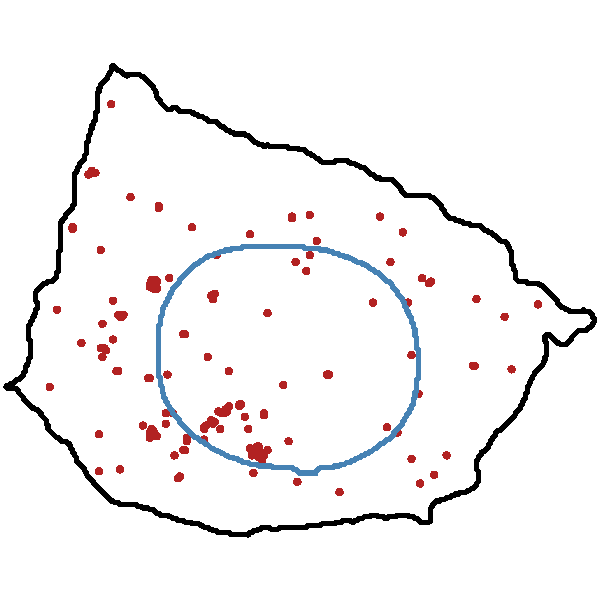
\includegraphics[width=\linewidth]{figures/introduction/real_coord_foci}
		\subcaption{Foci}
	\endminipage\hfill
	\minipage{0.2\textwidth}
		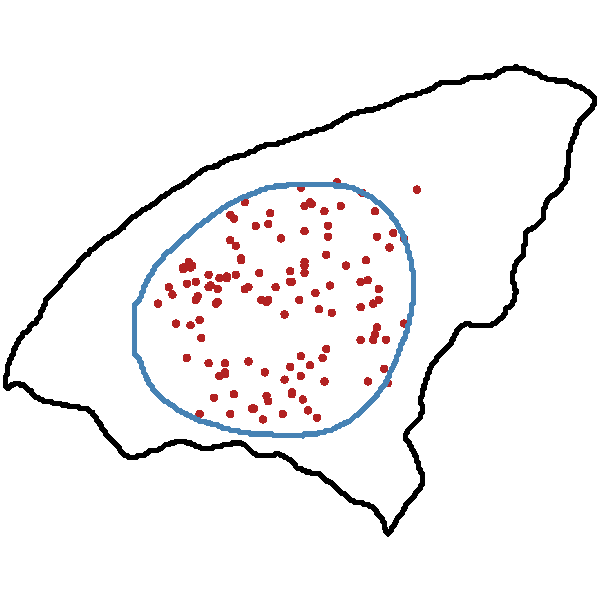
\includegraphics[width=\linewidth]{figures/introduction/real_coord_intranuclear}
		\subcaption{Intranuclear}
	\endminipage\hfill
	\minipage{0.2\textwidth}
		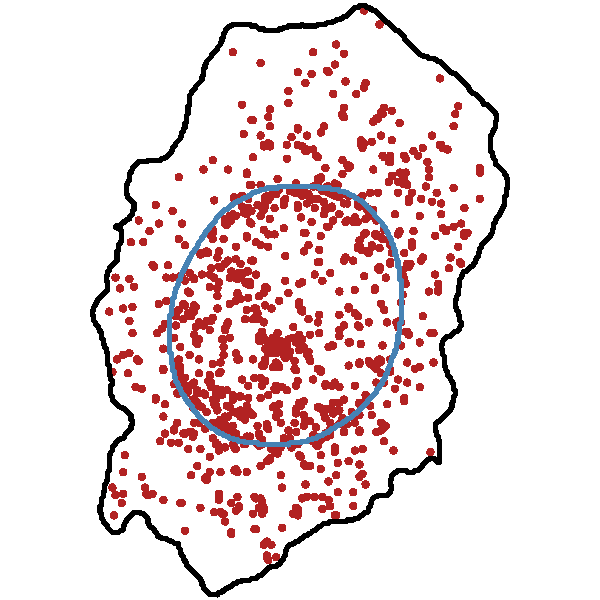
\includegraphics[width=\linewidth]{figures/introduction/real_coord_nuclear_edge}
		\subcaption{Nuclear edge}
	\endminipage\hfill
	\minipage{0.2\textwidth}
		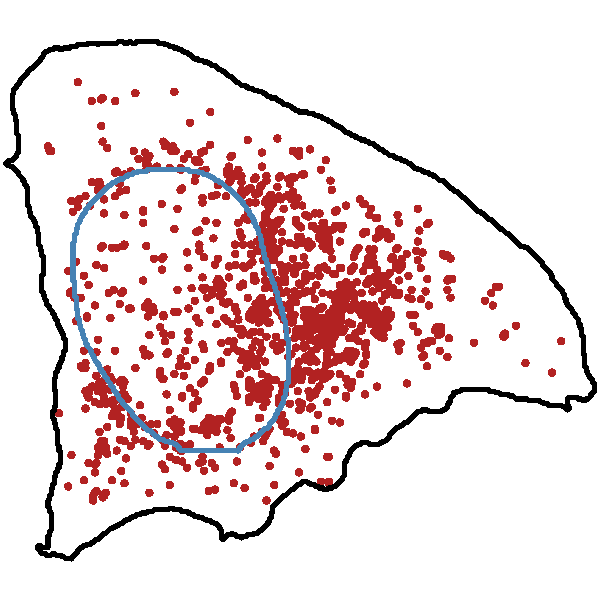
\includegraphics[width=\linewidth]{figures/introduction/real_coord_perinuclear}
		\subcaption{Perinuclear}
	\endminipage\hfill
	\minipage{0.2\textwidth}
		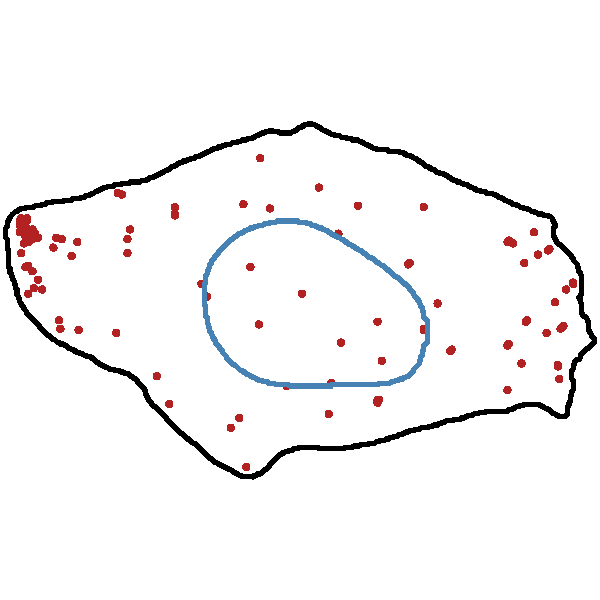
\includegraphics[width=\linewidth]{figures/introduction/real_coord_protrusion}
		\subcaption{Protrusion}
	\endminipage
	\caption{RNA localization patterns from~\cite{CHOUAIB_2020}.
	Coordinate representations with RNA spots (\textit{red}), cell membrane (\textit{black}) and nuclear membrane (\textit{blue}).
	Detection and segmentation results are extracted and visualized with \emph{bigfish}}
	\label{fig:localization_patterns_racha_features}
\end{figure}

\subsection{Results}
\label{subsec:results_general_pattern}

\subsubsection{Unsupervised visualization}

\subsubsection{Gene aggregated results}

%3.4 Unsupervised visualization
Another part of our work concerns the representation of thousands of cells
based on localization features. We adopt an unsupervised approach. From the
hand-crafted features or those built automatically by the neural network, we
have a representation of each cell in a multidimensional point cloud. We use
a t-distributed stochastic neighbour embedding (t-SNE) [38] to get a 2-dimensional
projection of such a point cloud. The algorithm computes the probability distribution
relative to the similarities of different observations in our high-dimensional
space and the same probability distribution for observations in a 2-dimensional
space. The 2-dimensional projection which minimizes the KL-divergence between
both distributions is returned. Figure 13 is a 2-dimensional projection of the
high-dimensional vectors returned by the neural network we describe in the
previous section. The point cloud represents 4,000 real cells extracted from
experimental images. Some clusters appear, especially for the foci, nuclear
retention and extension patterns. Examples of relative input images are given
in the figure. Different genes can present the same pattern. On the contrary,
a same gene can present heterogeneous patterns. For example, if most of the
time CEP192 mRNAs are kept inside the nucleus, they are periodically released
in the cytoplasm.

\section{Translation factories}
\label{sec:translation_factories}

\begin{center}
	\textit{(To be completed)}
\end{center}

\subsection{Introduction}
\label{subsec:introduction_translation_factories}

\subsection{Materials and methods}
\label{subsec:materials_translation_factories}

\subsubsection{Puromycin drug}

\subsubsection{Cluster detection}

\subsection{Results}
\label{subsec:results_translation_factories}

\section{Centrosomal pattern}
\label{sec:centrosomal}

\begin{center}
	\textit{(To be completed)}
\end{center}

\subsection{Introduction}
\label{subsec:introduction_centrosomal}

\subsection{Materials and methods}
\label{subsec:materials_centrosomal}

\subsubsection{Experimental data}

\subsubsection{Centrosome detection}

\subsubsection{Cell and nucleus segmentation}

\subsection{Results}
\label{subsec:results_centrosomal}

\subsubsection{Centrosomal mRNAs}

\subsubsection{Influence of mitosis}

\section{Protrusion pattern}
\label{sec:protrusion}

\begin{center}
	\textit{(To be completed)}
\end{center}

\subsection{Introduction}
\label{subsec:introduction_protrusion}

\subsection{Materials and methods}
\label{subsec:materials_protrusion}

\subsection{Results}
\label{subsec:results_protrusion}

\section{Exploring large scale dataset}
\label{sec:exploration}

\begin{center}
	\textit{(To be completed)}
\end{center}

%~\cite{lecuyer_global_2007}

To address this point, we developed and employed a high-resolution fluorescent
in situ hybridization procedure to comprehensively evaluate mRNA localization
dynamics during early Drosophila embryogenesis. Surprisingly, of the 3370 genes
analyzed, 71\% of those expressed encode subcellularly localized mRNAs.
Dozens of new and striking localization patterns were observed, implying an
equivalent variety of localization mechanisms. Tight correlations between mRNA
distribution and subsequent protein localization and function, indicate major
roles for mRNA localization in nucleating localized cellular machineries.

Computational Analysis The annotation data was converted into a binary matrix,
containing genes on one axis and localization terms on the other, where the presence
of a localization feature for a given gene was indicated numerically as ‘‘1,’’
while lack of a feature was annotated as ‘‘0.’’ This matrix was then used for GO
term enrichment analysis. Functional GO annotations for all genes were downloaded
from Flybase (http://flybase.bio. indiana.edu/genes/lk/function/). Annotations
were up-propagated using the GO hierarchy (Ashburner et al., 2000), and calculations
were restricted to genes that were both GO annotated and analyzed in this study
(1651 genes). The hypergeometric distribution was used to calculate probabilities
of overlap between each localization category against all GO categories containing
three or more genes. The Benjamini-Hochberg procedure (Benjamini and Hochberg, 1995)
was used to control for multiple testing by computing a P-value threshold
corresponding to a false discovery rate (FDR) of 0.25. Transcript subgroups
were also analyzed independently for GO term enrichments using EASE (Hosack et al., 2003).
EASE scores of less that 0.05 were considered significant, as reported previously (Tadros et al., 2007a).

\section{Conclusion}
\label{sec:conclusion_chapter5}

\begin{center}
	\textit{(To be completed)}
\end{center}